\documentclass[twocolumn]{article}
\usepackage[utf8]{inputenc}
\setlength{\columnsep}{1cm}
\usepackage{graphicx}
\graphicspath{ {images/} }
\title{DataRocks Midterm Report}
\author{Kevin Huang, Xinran Pan, Francis Yih }
\date{October 2016}

\begin{document}

\maketitle

\section{Introduction}
	The goal of DataRocks’s project is to use a Kaggle dataset containing character and number images from Google StreetView and map these images to output alphabetical and numerical values (lower, uppercase letters, and digits). By doing so, we hope to create a good image-to-text converter for practical applications. 
\section{DataSet}
    After carefully looking through our data, we realized we needed to make some initial modifications to our training dataset. Kaggle originally provided a few datasets to choose from, including a file for the actual image sizes as well as a file with resized images. We decided to use the resized, 20x20 *.bmp files as it standardizes the size of each image and provides features of the same size as well. 
\section{Feature Selection and Preprocessing}
    The next step was to read the pixel values from a *.bmp file, and in order to accomplish this, we used a python library (PIL -> Python Imaging Library) to read our file.This library gave us the handle we needed to perform basic features with the data and obtain the pixel data. When we saw the values the pixels took, we realized they were in the form of a 3-tuple. This RGB-tuple describes the color of each pixel, but a letter is equally distinguishable in black and white. Therefore, we turned all of the images into grey-scale. Now, instead of dealing with three values at each pixel, we only need one. The final part of this processing was to separate the data into a test and training set to estimate the out-of-sample errors. We have not yet separated out a validation set since we have not used regularized least-squares on our data. We then wrote the cleaned-up data into a *.csv file for easy data manipulations and imported both training and test files into Julia. 

\section{Julia DataFrames}
    We read both *.csv files as dataframes arrays in Julia. Each array has a “:File” with the corresponding file, “:Value” and “:1 $\rightarrow$ :400” representing the pixel data. In the “:Value” column of the training set, each uppercase/lowercase letter and number represents what the image’s letter or number is. In our separated training set, there are a total of 5055 images and 400 features for each image, with an image spanning 20 $\times$ 20 pixels. Each of the features contains a value from 0 to 255 where zero is black, 255 is white, and the values between them are a shade of grey. 

\section{Corrupted/Missing Data}
    In terms of missing or corrupted data, a quick glance at the cvs file does not provide information as to whether there is messy data. Every entry to each feature contains a pixel value. We can only find missing or corrupted data by looking at the actual image and observing whether the image is legible. Examples of illegible images include pixels which blur the character or off-center and cropped characters. We acknowledge that this is not an efficient or fool-proof method for finding messy data but it is the easiest approach for now. Overall, from the sample of images we looked at, there does not seem to exist many obscure images.
    \begin{figure}[ht]
    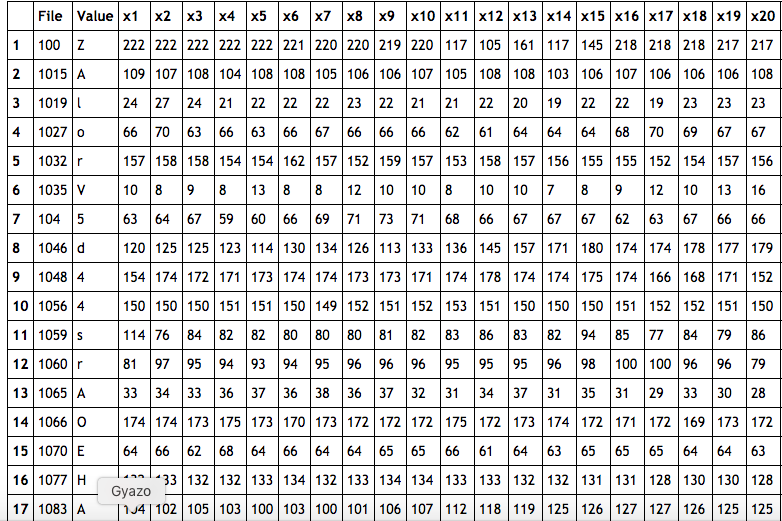
\includegraphics[width=8cm, height=6cm]{dataframeJulia}
    \caption{"DataFrame loaded into Julia"}
    \vspace{-0.7cm}
    \end{figure}
\section{Dataset Visualization}
    To get a better sense of the distribution of letters and numbers, we created a histogram of all 52 upper and lower case letters and 0 to 9 digits. This shows us which values we may have more or less of, and if we have enough data to properly classify each of the values.
    \par
    It turns out there is a large variance between the number of images we get for each character. We are not exactly sure how this may affect the results of any model we choose later on. It seems the characters with fewer number of images may be much harder to classify compared to characters with many number of images. 
	\begin{figure}[ht]
	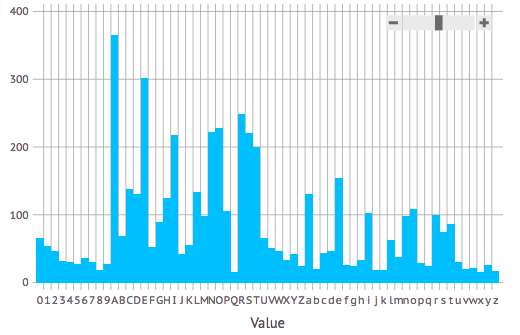
\includegraphics[width=8cm, height=6cm]{histogram}
	\end{figure}
\section{Simple Regression}
	We tried running a simple linear regression using all of our pixels as individual separate features. Our X matrix has the dimensions 5055 $\times$ 400, and our y vector has the dimensions 5055 $\times$ 1. We mapped all of the characters to a numerical value to give every letter a numerical representation. We did this using Julia’s character-to-integer conversion. However, the accuracy of the regression is terrible, even if tested with in-sample data (which should give artificially high accuracy). The percentage that our model got correct was $88/5055$, which is around $1.6\%$ accuracy.
	\par
	In conclusion, a simple linear regression does not make much sense for our model. Each picture is different, and there is not necessarily a linear correlation between each character. Due to the way we mapped each character to a number, we may have given them new characteristics. 
    \par
    With regards to over-fitting or under-fitting our model, we plan to use our test set to estimate the out-of-sample error. We do not think our models will ever under-fit, since we intend to use all of the data provided to gain a higher accuracy. We intend to prevent or minimize over- fitting by adding regularizers to the models we will create. In this case, we will further partition our data to have a validation set to choose the best $\lambda$ for our regularizer, then test it on the test data, and find the out-of-sample error. 
\section{Future Plans}
    Since we have only tried modeling our data with a simple linear regression, we still have many ideas to try. Some concepts we would like to further experiment with are clustering or neural network models which could help make better classifications.
    \subsection{Clustering}
    We can possibly train a better model for classifying our images by using some clustering algorithms. These algorithms help us determine which points are close to each other in terms of pixel value. By determining how close each point is with each other, we can assign them into different clusters of points. With different cluster patterns, we should be able to identify and classify which shape it falls under.
    \subsection{Neural Networks}
    Another approach that we would like to try is to be able to classify these images with a neural network. A neural network is made out of layers of artificial nodes called "neurons" that take the pixel values as input and transforms them into an output value. This transformation is non-linear and should be able to help us turn our pixel data into something that our images would be able to map to.
    \subsection{Further Feature Selection}
    Lastly, we can think about more creative feature selection and transformations on our data in order to help our models become even better. We might think about centering the characters in an image in a certain way, or smoothing/enhancing the image to have better contrasts and less noise within the picture. We can perhaps see whether changing the intensity of the colors (i.e. turning more of the pixels with values close to 0 into 0 and vice-versa), will affect the accuracy of our models.
\section{Considerations}
    We have a lot of interesting ideas that we are quite keen to try out. This may lead us to have more options that we have time to try out. We intend to focus on at least being able to have a simple clustering model and neural network model by the end of the project, by focusing on these two ideas. We also need to take into consideration the way we deal with the balance between variance and bias within these models. We need to research into these models and their respective loss functions. We would also would want to create better graphics in order to analyze our data better, such as graphics that show us the variance between pixels within our images that correspond with the same character.
\section{Conclusion}
    We have started working on our dataset, cleaned the data and exported it to Julia to work with. Currently we are working on developing a model that will be able to classify our data with a high accuracy. We plan to try different approaches in order to figure out which model describes the data best, and then refine the model with regularizers.

\end{document}
